% Réseau de neurones à deux couches cachées -> ../reseau.svg
% Compilation : sh build.sh
\documentclass[tikz,border=4pt]{standalone}
\definecolor{hearcred}{HTML}{FF0000}
\definecolor{hearcgray}{HTML}{6E6E6E}
\begin{document}
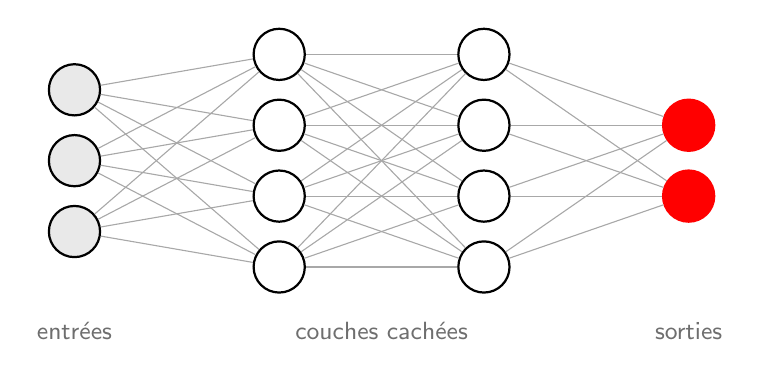
\begin{tikzpicture}[
    x=2.6cm, y=0.9cm,
    neurone/.style={circle, draw=black, line width=0.8pt, minimum size=0.65cm},
    entree/.style={neurone, fill=hearcgray!15},
    cache/.style={neurone, fill=white},
    sortie/.style={neurone, fill=hearcred, draw=hearcred},
    lien/.style={hearcgray!60, line width=0.4pt},
  ]
  \foreach \i in {1,...,3} \node[entree] (e\i) at (0, 2-\i) {};
  \foreach \i in {1,...,4} \node[cache]  (a\i) at (1, 2.5-\i) {};
  \foreach \i in {1,...,4} \node[cache]  (b\i) at (2, 2.5-\i) {};
  \foreach \i in {1,...,2} \node[sortie] (s\i) at (3, 1.5-\i) {};

  \foreach \i in {1,...,3} \foreach \j in {1,...,4} \draw[lien] (e\i) -- (a\j);
  \foreach \i in {1,...,4} \foreach \j in {1,...,4} \draw[lien] (a\i) -- (b\j);
  \foreach \i in {1,...,4} \foreach \j in {1,...,2} \draw[lien] (b\i) -- (s\j);

  \begin{scope}[font=\sffamily\small, text=hearcgray]
    \node at (0, -2.4) {entrées};
    \node at (1.5, -2.4) {couches cachées};
    \node at (3, -2.4) {sorties};
  \end{scope}
\end{tikzpicture}
\end{document}
